\documentclass[12pt,a4paper]{article}

\usepackage[utf8]{inputenc}
\usepackage[T1]{fontenc}
\usepackage[croatian]{babel}   % latinicni jezik s dijakriticima (c, c, z, s, dj)
\usepackage[a4paper,margin=2.5cm]{geometry}
\usepackage{amsmath}
\usepackage{amssymb}
\usepackage{graphicx}
\usepackage{booktabs}
\usepackage{siunitx}
\usepackage{float}
\usepackage[hidelinks]{hyperref}

\graphicspath{{figures/}}

\title{\textbf{Proračun kratkih spojeva za transmisione mreže\\(simetrične mreže)}}
\author{Ilhan Erović\\[4pt]\normalsize Univerzitet u Sarajevu --- Elektrotehnički fakultet\\
\normalsize Seminarski rad iz predmeta SREES}
\date{2026}

\begin{document}
\maketitle

\begin{abstract}
\noindent U radu je opisan proračun simetričnih (tropolnih) kratkih spojeva u
transmisionim mrežama i implementiran samostalni program s grafičkim interfejsom
zasnovan na frameworku \emph{natID}. Program učitava opis mreže u MATPOWER
\texttt{.m} formatu, formira matricu admitansi $\mathbf{Y}_{\text{bus}}$ kao
rijetku kompleksnu matricu, te \emph{Z-bus} metodom računa struju kvara, napone
svih sabirnica poslije kvara, struje kroz grane i doprinos pojedinih generatora.
Rezultati su verifikovani poređenjem s nezavisnim proračunom u MATLAB-u
($\mathbf{Z}=\mathbf{Y}^{-1}$) i pokazuju potpuno slaganje.
\end{abstract}

\section{Uvod}
Kratki spoj je jedan od najtežih poremećaja u elektroenergetskom sistemu. Pri
kratkom spoju dolazi do naglog porasta struje i pada napona, što može oštetiti
opremu i ugroziti stabilnost sistema. Proračun kratkih spojeva je stoga osnova za
dimenzionisanje prekidača, podešavanje relejne zaštite i provjeru termičke i
dinamičke izdržljivosti opreme.

Ovaj rad se bavi \emph{simetričnim} kvarom --- tropolnim kratkim spojem u kojem su
sve tri faze simetrično zahvaćene. Zbog simetrije, analiza se svodi na
jednofazni ekvivalent (direktni/pozitivni redoslijed), pa nije potrebno
razlaganje na simetrične komponente. Cilj rada je razviti program koji za
proizvoljnu transmisionu mrežu (zadanu u MATPOWER formatu) izračunava sve
relevantne veličine kratkog spoja i prikazuje ih tabelarno i grafički.

\section{Teorijska osnova}

\subsection{Sistem jediničnih vrijednosti (per unit)}
Svi proračuni se izvode u sistemu jediničnih vrijednosti (\emph{per unit}, pu),
s bazom snage $S_b = \SI{100}{MVA}$ i baznim naponom svake naponske razine
$U_b$. Bazna struja i bazna impedansa su
\begin{equation}
I_b = \frac{S_b}{\sqrt{3}\,U_b}, \qquad Z_b = \frac{U_b^2}{S_b}.
\end{equation}

\subsection{Matrica admitansi $\mathbf{Y}_{\text{bus}}$}
Mreža se opisuje matricom admitansi sabirnica $\mathbf{Y}_{\text{bus}}$
dimenzije $N\times N$ ($N$ --- broj sabirnica). Za svaku granu (vod ili
transformator) između sabirnica $f$ i $t$, sa serijskom impedansom $r+jx$,
polovinom otočnog punjenja voda $b/2$, prijenosnim odnosom (tap) $\tau$ i faznim
pomakom $\theta$, definiše se
\begin{equation}
y = \frac{1}{r+jx}, \qquad a = \tau\,e^{j\theta},
\end{equation}
a doprinosi grane matrici $\mathbf{Y}_{\text{bus}}$ su:
\begin{align}
Y_{ff} &\mathrel{+}= \frac{y + j\tfrac{b}{2}}{a\,a^{*}}, &
Y_{tt} &\mathrel{+}= y + j\tfrac{b}{2},\\
Y_{ft} &\mathrel{+}= -\frac{y}{a^{*}}, &
Y_{tf} &\mathrel{+}= -\frac{y}{a}.
\end{align}
Otočni elementi sabirnica (kondenzatori/reaktori) dodaju se na dijagonalu:
$Y_{ii}\mathrel{+}=(G_s+jB_s)/S_b$.

\subsection{Model generatora}
Da bi proračun kratkog spoja imao fizičkog smisla, generatori se modeliraju kao
naponski izvori iza reaktanse prema referentnoj (uzemljenoj) tački. Svaki
generator na sabirnici $g$ doprinosi dijagonali otočnom admitansom
\begin{equation}
y_g = \frac{1}{j X'_d},
\end{equation}
gdje je $X'_d$ (tranzijentna reaktansa) na sistemskoj bazi. Prema podacima
korištenim u istraživanju (WSCC / Sauer--Pai), podrazumijevana vrijednost je
$X'_d = 0{,}0608$ pu, uz mogućnost zadavanja vrijednosti po pojedinom generatoru.

\subsection{Z-bus metoda proračuna kvara}
Impedantna matrica je inverz matrice admitansi,
$\mathbf{Z}_{\text{bus}}=\mathbf{Y}_{\text{bus}}^{-1}$. Umjesto pune inverzije,
za kvar na sabirnici $k$ rješava se linearni sistem
\begin{equation}
\mathbf{Y}_{\text{bus}}\,\mathbf{z} = \mathbf{e}_k,
\end{equation}
gdje je $\mathbf{e}_k$ jedinični vektor; rješenje $\mathbf{z}$ je $k$-ta kolona
matrice $\mathbf{Z}_{\text{bus}}$, a $Z_{kk}=z_k$ je vlastita (driving-point)
impedansa sabirnice kvara. Uz pretpostavku ravnog prednapona $V_0=1{,}0$ pu i
impedanse kvara $Z_f$, struja kvara je
\begin{equation}
I_f = \frac{V_0}{Z_{kk}+Z_f},
\end{equation}
a naponi svih sabirnica poslije kvara
\begin{equation}
V_i = V_0 - z_i\,I_f .
\end{equation}
Struja kroz granu $i\!\to\!j$ dobija se iz razlike napona:
$I_{ij} = y\,(V_i/a - V_j)$. Doprinos pojedinog generatora struji kvara je
\begin{equation}
I_g = \frac{E - V_g}{j X'_d}, \qquad E \approx V_0,
\end{equation}
gdje je $V_g$ napon na sabirnici generatora poslije kvara. Snaga kratkog spoja
na sabirnici $k$ je $S_k = \sqrt{3}\,U_b\,I_{f,\text{kA}} = S_b\,|I_f|_{\text{pu}}$.

\section{Metodologija i algoritam}
Algoritam proračuna prikazan je na slici~\ref{fig:flow}. Koraci su:
\begin{enumerate}
  \item učitavanje i parsiranje MATPOWER \texttt{.m} datoteke (sabirnice,
  generatori, grane);
  \item formiranje $\mathbf{Y}_{\text{bus}}$ (grane, otočni elementi, generatori
  kao reaktanse);
  \item faktorizacija $\mathbf{Y}_{\text{bus}}$ (rijetka LU dekompozicija);
  \item za odabranu sabirnicu kvara $k$: rješavanje $\mathbf{Y}\mathbf{z}=\mathbf{e}_k$,
  te računanje $I_f$, napona, struja grana i doprinosa generatora;
  \item prikaz rezultata (tabele, grafici, jednopolna shema) i izvoz.
\end{enumerate}

\begin{figure}[H]
  \centering
  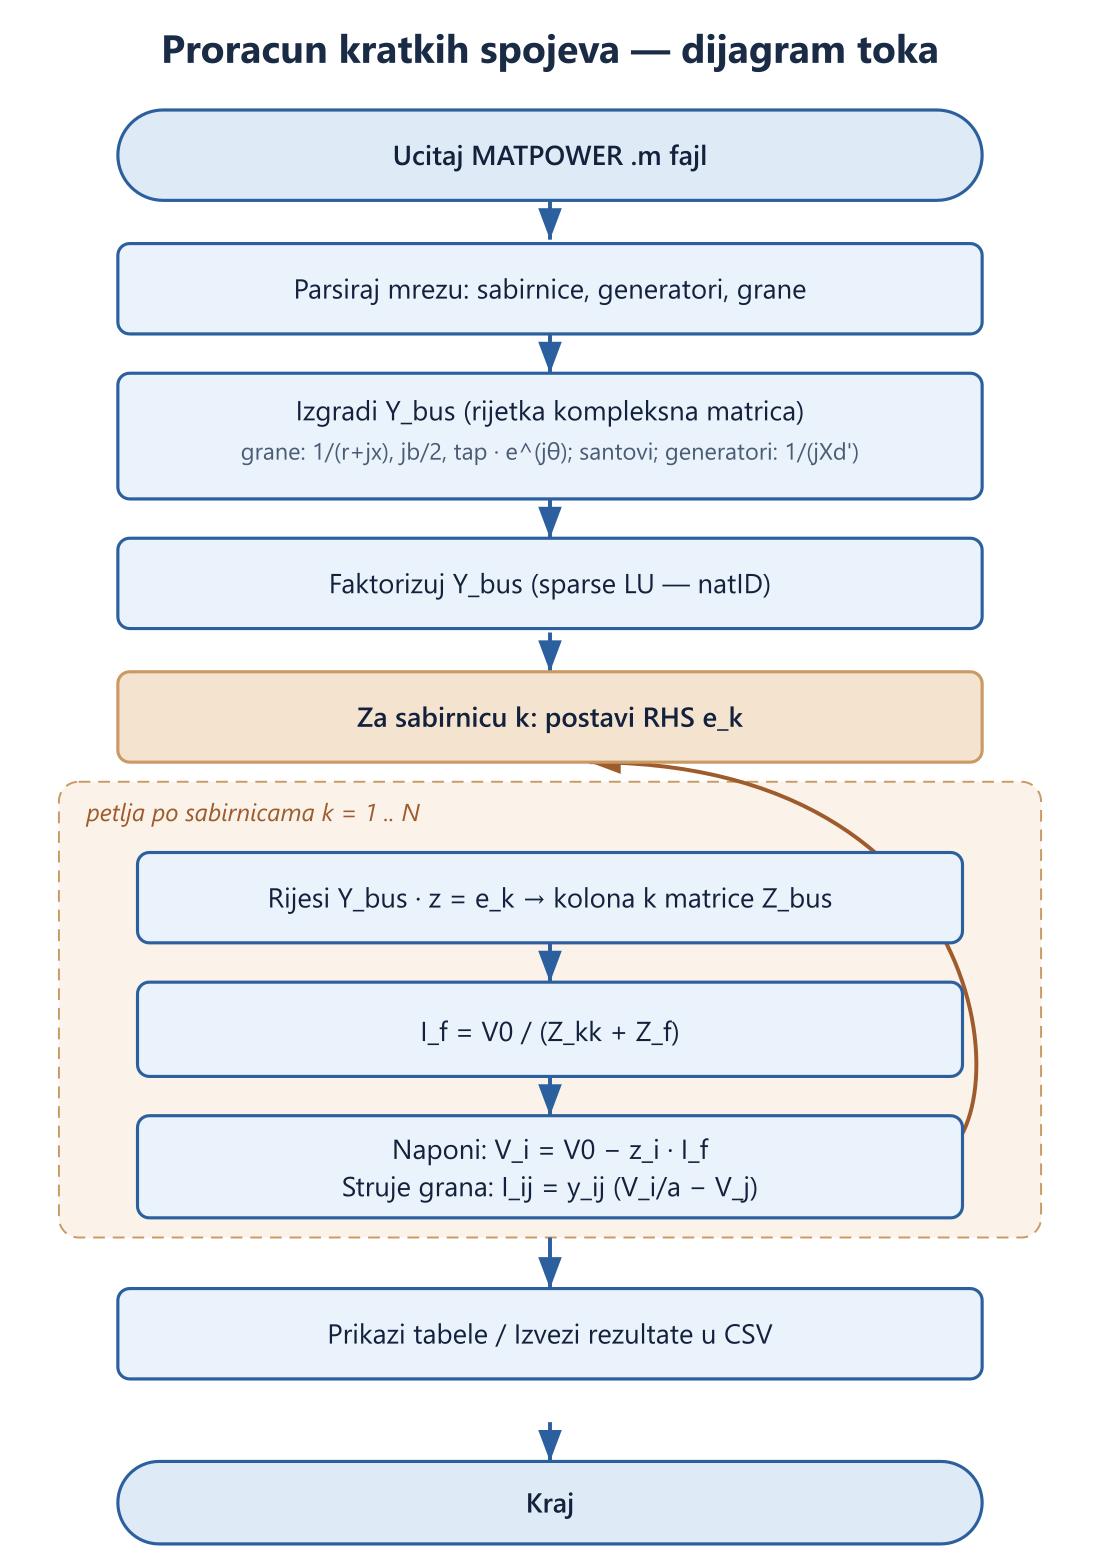
\includegraphics[width=0.52\textwidth]{flowchart.png}
  \caption{Dijagram toka algoritma proračuna kratkog spoja.}
  \label{fig:flow}
\end{figure}

\section{Implementacija}
Program je razvijen u jeziku \textbf{C++} korištenjem frameworka \textbf{natID}.
Jedina matrica u proračunu --- matrica admitansi $\mathbf{Y}_{\text{bus}}$ ---
realizovana je kao natID \emph{rijetka kompleksna} matrica
(\texttt{sparse::CmplxSolver}). Rijetka LU faktorizacija se izvodi jednom, a
zatim se za svaku sabirnicu kvara ponovo koristi (mijenja se samo desna strana
sistema), što je računski efikasno. Vektori rezultata (naponi, struje) čuvaju se
u standardnim kontejnerima.

Programska struktura je podijeljena na računsku jezgru (odvojenu od interfejsa) i
grafički interfejs:
\begin{itemize}
  \item \texttt{MatpowerParser} --- parsiranje \texttt{.m} formata;
  \item \texttt{ShortCircuitSolver} --- formiranje $\mathbf{Y}_{\text{bus}}$,
  faktorizacija i proračun kvara, struja grana i doprinosa generatora;
  \item GUI (\texttt{MainView} i pomoćne klase) --- unos parametara, tabovi s
  rezultatima, grafici i jednopolna shema crtani preko natID \texttt{Canvas}-a.
\end{itemize}
Projekat je konfigurisan u \textbf{CMake}-u (Windows i Linux). Interfejs
podržava učitavanje mreže, izbor sabirnice kvara, zadavanje reaktanse
generatora $X'_d$ i impedanse kvara $Z_f$, te izvoz rezultata u CSV i slika u
PDF/SVG. Slika~\ref{fig:gui} prikazuje glavni prozor s tabelom nivoa kvara.

\begin{figure}[H]
  \centering
  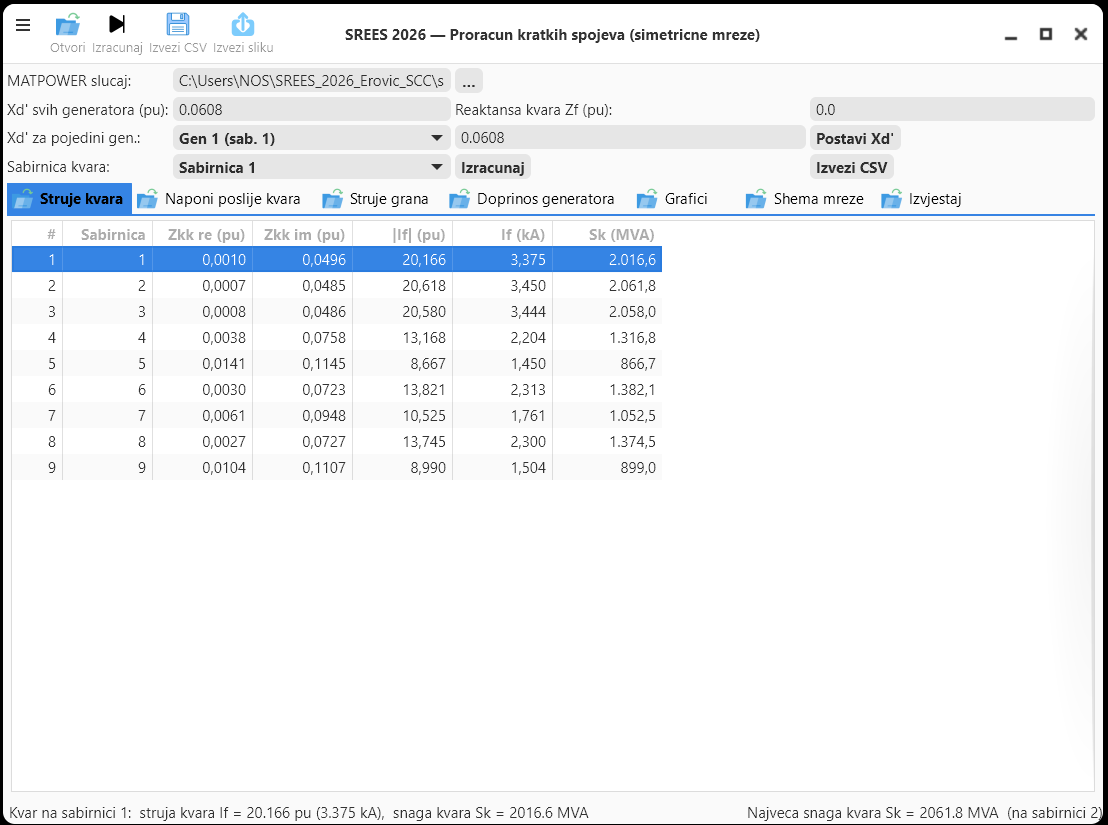
\includegraphics[width=0.9\textwidth]{gui_fault_table.png}
  \caption{Grafički interfejs: nivoi kvara po sabirnicama (test mreža case9).}
  \label{fig:gui}
\end{figure}

\section{Rezultati}
Program je testiran na standardnim MATPOWER mrežama (case5, case9, case30,
case118, case300). Kao primjer prikazani su rezultati za mrežu \textbf{case9}
(WSCC 9 sabirnica, 3 generatora) pri tropolnom kvaru na sabirnici~1
($X'_d=0{,}0608$ pu, $Z_f=0$, ravni prednapon).

\begin{table}[H]
  \centering
  \caption{Nivoi kvara po sabirnicama --- case9 (tropolni kvar zasebno na svakoj sabirnici).}
  \label{tab:fault}
  \begin{tabular}{crrr}
    \toprule
    Sabirnica & $|I_f|$ (pu) & $I_f$ (kA) & $S_k$ (MVA)\\
    \midrule
    1 & 20{,}166 & 3{,}375 & 2016{,}6\\
    2 & 20{,}618 & 3{,}450 & 2061{,}8\\
    3 & 20{,}580 & 3{,}444 & 2058{,}0\\
    4 & 13{,}168 & 2{,}204 & 1316{,}8\\
    5 &  8{,}667 & 1{,}450 &  866{,}7\\
    6 & 13{,}821 & 2{,}313 & 1382{,}1\\
    7 & 10{,}525 & 1{,}761 & 1052{,}5\\
    8 & 13{,}745 & 2{,}300 & 1374{,}5\\
    9 &  8{,}990 & 1{,}504 &  899{,}0\\
    \bottomrule
  \end{tabular}
\end{table}

Za kvar na sabirnici~1 struja kvara iznosi $I_f = 20{,}166$ pu $=3{,}375$ kA, a
snaga kratkog spoja $S_k = 2016{,}6$ MVA. Doprinosi generatora dati su u
tabeli~\ref{tab:gen}: generator na samoj sabirnici kvara (G1) daje najveći dio
struje (79{,}1\,\%), dok udaljeni generatori (G2, G3) doprinose po 10{,}5\,\%.

\begin{table}[H]
  \centering
  \caption{Doprinos generatora struji kvara --- case9 (kvar na sabirnici 1).}
  \label{tab:gen}
  \begin{tabular}{crrr}
    \toprule
    Generator (sabirnica) & $|I|$ (pu) & $|I|$ (kA) & \% doprinosa\\
    \midrule
    1 & 16{,}447 & 2{,}752 & 79{,}1\\
    2 &  2{,}176 & 0{,}364 & 10{,}5\\
    3 &  2{,}177 & 0{,}364 & 10{,}5\\
    \bottomrule
  \end{tabular}
\end{table}

Slika~\ref{fig:charts} prikazuje grafike snage kvara po sabirnicama i profil
napona poslije kvara, a slika~\ref{fig:oneline} jednopolnu shemu mreže na kojoj
su bojom označeni naponi sabirnica, a debljinom grana struje kroz njih.

\begin{figure}[H]
  \centering
  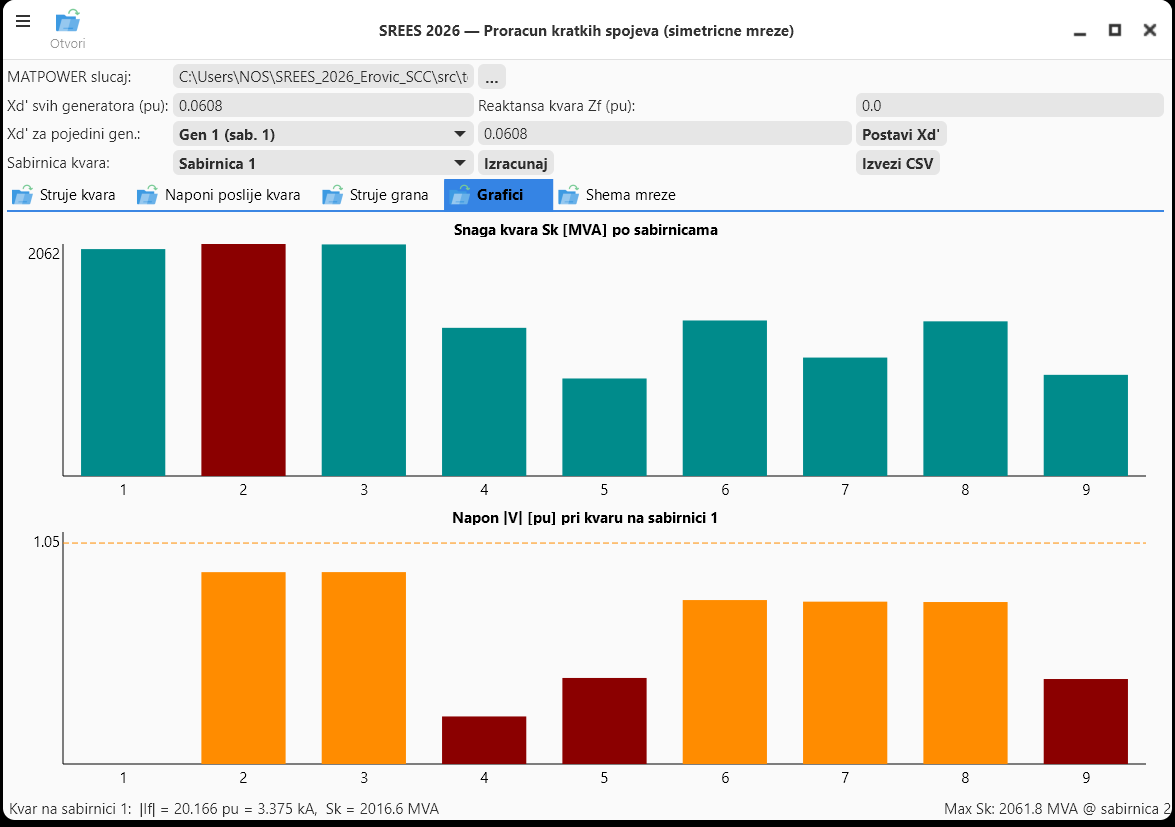
\includegraphics[width=0.92\textwidth]{charts.png}
  \caption{Snaga kratkog spoja $S_k$ po sabirnicama i profil napona $|V|$
  (kvar na sabirnici 1).}
  \label{fig:charts}
\end{figure}

\begin{figure}[H]
  \centering
  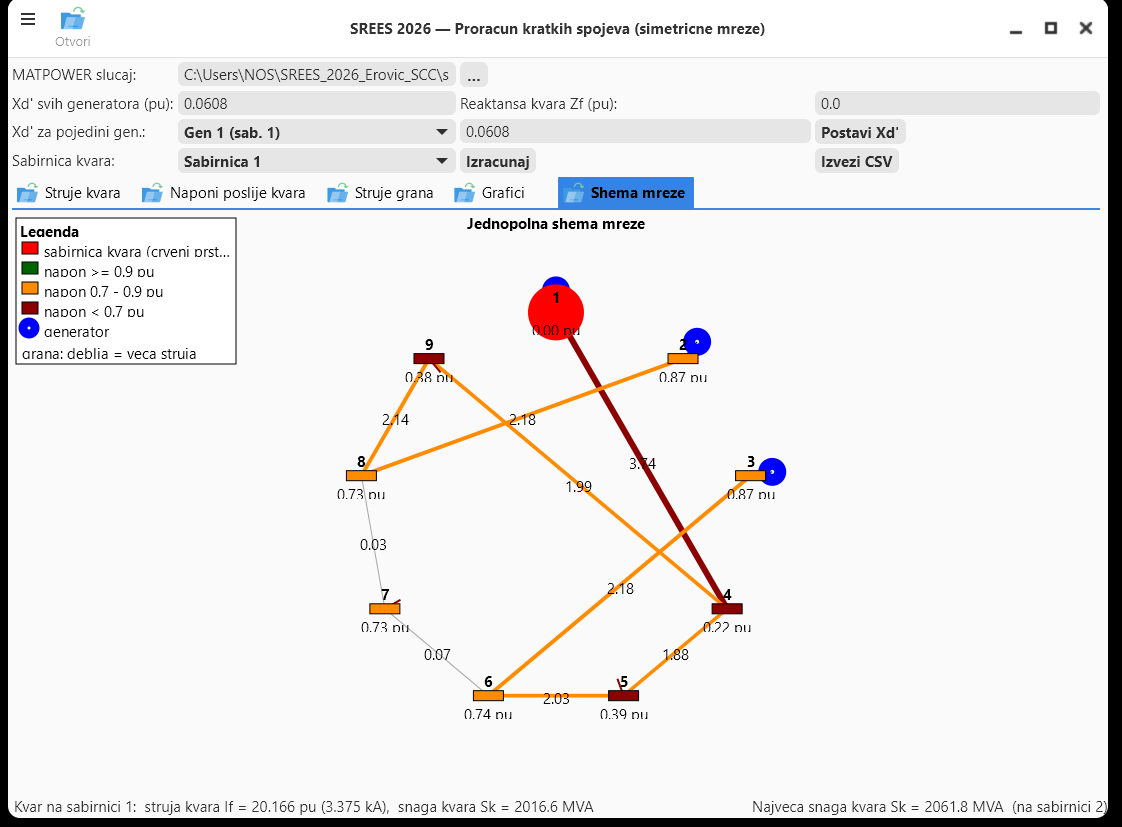
\includegraphics[width=0.85\textwidth]{oneline_app.png}
  \caption{Jednopolna shema mreže case9 s rezultatima kvara: crvena sabirnica =
  mjesto kvara, boja = napon, debljina grane = struja.}
  \label{fig:oneline}
\end{figure}

\subsection{Verifikacija}
Tačnost proračuna provjerena je nezavisno u MATLAB-u, formiranjem iste matrice
$\mathbf{Y}_{\text{bus}}$ i računanjem $\mathbf{Z}_{\text{bus}}=\mathbf{Y}^{-1}$
(puna inverzija). Vrijednosti $Z_{kk}$, struje kvara i struja grana dobijene
programom poklapaju se s MATLAB referencom do na četiri decimalna mjesta za sve
sabirnice, čime je potvrđena ispravnost implementacije.

\section{Zaključak}
Razvijen je funkcionalan i verifikovan program za proračun simetričnih kratkih
spojeva u transmisionim mrežama. Program koristi Z-bus metodu i rijetke
kompleksne matrice iz natID frameworka, čime postiže efikasnost i na velikim
mrežama (do 300 sabirnica). Pored numeričkih rezultata (struje kvara, naponi,
struje grana, doprinos generatora), program nudi grafičku vizualizaciju i izvoz
rezultata, što ga čini pogodnim kako za inženjersku upotrebu tako i za nastavne
svrhe.

\begin{thebibliography}{9}
\bibitem{kundur} P. Kundur, \emph{Power System Stability and Control}, McGraw-Hill, 1994.
\bibitem{sauerpai} P.\,W. Sauer, M.\,A. Pai, \emph{Power System Dynamics and Stability}, 2007.
\bibitem{matpower} R.\,D. Zimmerman, C.\,E. Murillo-Sánchez, R.\,J. Thomas,
``MATPOWER: Steady-State Operations, Planning and Analysis Tools,''
\emph{IEEE Trans. Power Systems}, vol.~26, no.~1, 2011.
\bibitem{grainger} J.\,J. Grainger, W.\,D. Stevenson, \emph{Power System Analysis}, McGraw-Hill.
\bibitem{natid} I. Džafić, \emph{natID --- native Interface Design framework}, \url{https://github.com/idzafic/natID}.
\end{thebibliography}

\end{document}
